\documentclass[border=3pt]{standalone}
% Preâmbulo compartilhado pelos diagramas TikZ da aula 7 de IHC (Organização do Espaço de Problema)
\usepackage[T1]{fontenc}
\usepackage[utf8]{inputenc}
\usepackage{lmodern}
\usepackage{amsmath}
\usepackage{xcolor}
\usepackage{tikz}
\usetikzlibrary{arrows.meta,angles,quotes,decorations.pathmorphing,calc,
                positioning,shapes.geometric,shapes.misc,backgrounds,fit,
                math}

% Paleta (mesma dos SVGs originais)
% Paleta da disciplina de IHC: acento roxo (#755099), da capa do livro.
% (o nome "dblue" é mantido para não alterar todos os diagramas)
\definecolor{dblue}{HTML}{755099}
\definecolor{dorange}{HTML}{B3541E}
\definecolor{dgreen}{HTML}{4A7C59}
\definecolor{dred}{HTML}{9C4B4B}
\definecolor{dcream}{HTML}{F4F1EA}
\definecolor{dshade}{HTML}{DDD7C9}

% Função gaussiana (não normalizada por padrão de escala visual)
\pgfmathdeclarefunction{gauss}{3}{%
  \pgfmathparse{1/(#3*sqrt(2*pi))*exp(-((#1-#2)^2)/(2*#3^2))}%
}

% Estilos comuns (prefixo d... para não colidir com chaves internas do pgf)
\tikzset{
  >={Stealth[length=2mm]},
  dguide/.style={gray!55, dashed, line width=0.4pt},
  daxis/.style={gray!60, line width=0.7pt, ->},
  dbody/.style={fill=black!3, draw=black!80, line width=1pt},
  dacc/.style={draw=dblue, line width=1pt},
  dlbl/.style={black!55, font=\small},
  dsub/.style={black!45, font=\footnotesize},
  dstate/.style={circle, draw=black!80, fill=dcream, line width=1pt,
                 minimum size=17mm, font=\large, inner sep=1pt},
  dobs/.style={circle, draw=black!80, fill=dshade, line width=1pt,
               minimum size=14mm, font=\large, inner sep=1pt},
  dbox/.style={rounded corners=2pt, draw=black!80, fill=dcream, line width=1pt,
               align=center, inner sep=6pt},
  dop/.style={circle, draw=black!80, fill=white, line width=1pt,
              minimum size=6mm, inner sep=0pt, font=\small},
  dtrans/.style={->, dblue, line width=1pt},
  dmeas/.style={->, dorange, line width=1pt},
  dcurve/.style={line width=1pt, dblue},
  dcurveb/.style={line width=1.4pt, dorange},
}

\begin{document}
\hyphenpenalty=10000 \exhyphenpenalty=10000 \tolerance=9999 \emergencystretch=3em
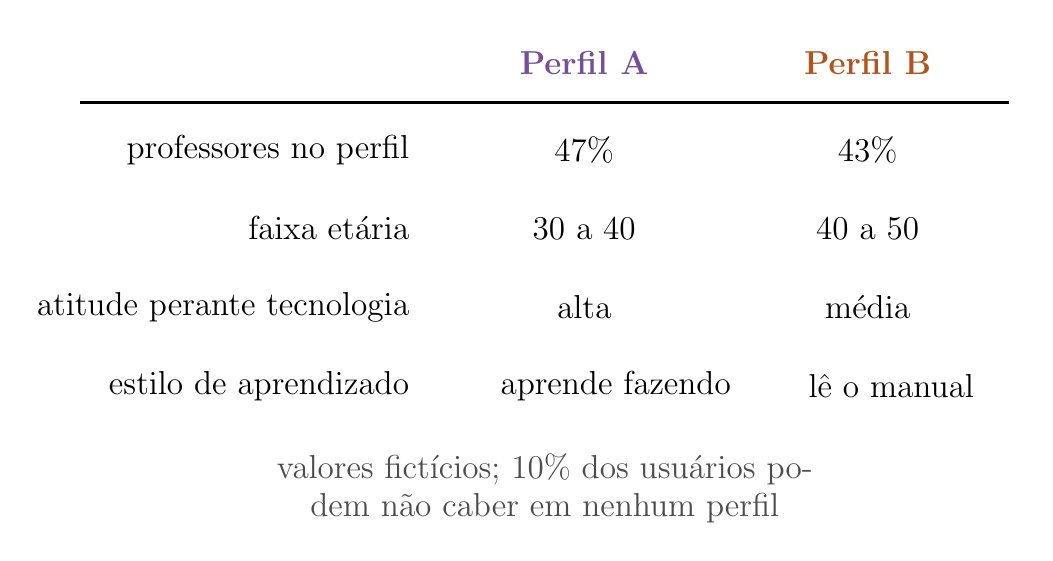
\begin{tikzpicture}[x=1cm,y=1cm]
  \tikzset{h/.style={font=\large\bfseries, minimum height=0.9cm, minimum width=3.4cm, align=center}, v/.style={font=\large, minimum height=0.9cm, minimum width=3.4cm, align=center}, l/.style={font=\large, anchor=east}}
  \node[h, text=dblue] at (6.0,5.6) {Perfil A};
  \node[h, text=dorange] at (9.6,5.6) {Perfil B};
  \draw[line width=1.2pt] (-0.4,5.1) -- (11.4,5.1);
  \node[l] at (3.9,4.5) {professores no perfil};  \node[v] at (6.0,4.5) {47\%}; \node[v] at (9.6,4.5) {43\%};
  \node[l] at (3.9,3.5) {faixa etária};  \node[v] at (6.0,3.5) {30 a 40}; \node[v] at (9.6,3.5) {40 a 50};
  \node[l] at (3.9,2.5) {atitude perante tecnologia};  \node[v] at (6.0,2.5) {alta}; \node[v] at (9.6,2.5) {média};
  \node[l] at (3.9,1.5) {estilo de aprendizado};  \node[v] at (6.4,1.5) {aprende fazendo}; \node[v] at (9.9,1.5) {lê o manual};
  \node[font=\large, black!70, text width=11cm, align=center] at (5.5,0.2) {valores fictícios; 10\% dos usuários podem não caber em nenhum perfil};
\end{tikzpicture}
\end{document}
